% !TEX encoding = UTF-8 Unicode
\documentclass[12pt,a4paper,english
% ,twoside,openright
]{tunithesis}

\special{papersize=210mm,297mm}

\author{Roosa Kuusivaara \& Väinö-Waltteri Granat}
\title{Characterizing holographic displays via
numerical simulations - Report} % primary title (for front page)
\thesistype{Laboratory Report} % or Bachelor of Science, Laboratory Report...

\usepackage{lastpage}
\usepackage[english]{babel}
\usepackage[
backend=biber,
style=numeric,
citestyle=numeric,
autocite=inline
]{biblatex}
\usepackage{csquotes}
\usepackage{mathrsfs, amsmath}

\addbibresource{references.bib} %Imports bibliography file


\definecolor{tunipurple}{RGB}{78, 0, 142}

\newcommand\todo[1]{{\color{red}!!!TODO: #1}} % Remark text in braces appears in red
\newcommand{\angs}{\textsl{\AA}}              % , e.g. slanted symbol for Ångstöm
% Preparatory content ends here


\pagenumbering{roman} % was: {Roman}
\pagestyle{headings}
\begin{document}

% Special trick so that internal macros (denoted with @ in their name)
% can be used outside the cls file (e.g. \@author)
\makeatletter

% Create the title page.
% First the logo. Check its language.
\thispagestyle{empty}
\vspace*{-.5cm}\noindent

\begin{figure}
    \vspace{-1.3cm}
    \advance\leftskip-2.5cm
    \noindent
\includegraphics{img/tunilogo.png}
\end{figure}
 
\vspace{2.5cm}
\begin{flushright}
\noindent\textsf{\LARGE{\@author}}

\noindent\vspace{0.5cm}

\noindent\Huge{\textsf{\textbf{\textcolor{tunipurple}{\@title}}}}
\end{flushright}
\vspace{13.7cm} % adjust to 12.7 this if thesis title needs two lines

% Last some additional info to the bottom-right corner
\begin{flushright}  
    \begin{spacing}{1.0}
      \textsf{Faculty of Information Technology and Communication Sciences (ITC)\\
      \@thesistype\\}
    \end{spacing}
\end{flushright}

% Leave the backside of title page empty in twoside mode
\if@twoside
\clearpage
\fi

% Turn off page numbering for the first pages
\pagenumbering{gobble}


% Some fields in abstract are automated, namely those with \@ (author,
% title, thesis type).
\chapter*{Abstract}
\begin{spacing}{1.0}
\noindent \@author: \@title\\
\@thesistype\\
Tampere University\\
Master’s Degree Programme in Signal Processing\\
October 2023 \\
\end{spacing}
\noindent\rule{12cm}{0.4pt}

\vspace{0.5cm}

% ---------------------------------------
% Abstract and keywords
% ---------------------------------------

\noindent
This is document is a laboratory report for work done for Advanced Signal Processing Laboratory course in the Characterizing holographic displays via numerical simulations assignment. The work consisted about implementing Fresnel and Rayleigh-Sommerfield synthesis methods to an exisiting field wave propagation based 1D hologram simulations, as well as analysis done for the viewing results produced by these and Holographic Stereopgram based synthesis. Analysis focused on finding the optimal focal length for each of the synthesis methods by calculating MTF values for produced images, with different focal lenghts and fitting a function to these values.

~

\noindent\textbf{Keywords:} Laboratory Report, Holograms, Fresnel, Rayleigh-Sommerfield, Field wave propagation

~


% Add the table of contents


\setcounter{tocdepth}{3}              % How many header level are included
\tableofcontents                      % Create TOC


% The actual text begins here and page numbering changes to 1,2...
% Leave the backside of title empty in twoside mode
\if@twoside
%\newpage
\cleardoublepage
\fi


\renewcommand{\chaptername}{} % This disables the prefix 'Chapter' or
                              % 'Luku' in page headers (in 'twoside'
                              % mode)


\chapter{Introduction}
\label{ch:intro}
\pagenumbering{arabic}
\setcounter{page}{1} 
In this report we describe our work with the `Characterizing holographic displays via
numerical simulations` exercise, for the Advanced Signal Processing Laboratory Course~\cite{labassignment}.

In this project we familiarized ourselves with the basics of holographic display, by implementing a part of a holographics display viewing simulation. We implemented two holographic synthesis methods and a retinal image formation model, by contributing code to a MATLAB codebase given by the course faculty.

\section{Hologram synthesis}
Hologram synthesis describes the method for forming holographic images in 3d space from a given image. In this assignment, instead of using entire 3d space, the analysis can be simplified by considering only a cross section of the 3d space. The hologram is now represented as a 1D array of complex values. This simplification eases the computational load and also makes the process easier to handle.

\section{Retinal Image Formation}
In the study of holographic displays and their numerical characterization, Retinal Image Formation is a key part of the analysis. This simulation mimics how the human eye perceives visual information. Through this model, we obtain images on the retina, which can be used to analyze the perceived sharpness of the displayed content.

In these simulation tools, the human eye is considered as a camera, with the lens (the pupil) and the retina (the sensor). This simulation involves three key planes: the display (hologram), the lens, and the sensor. We model the pupil as a thin lens with a specific width, influencing how light passes through it.



\chapter{Methodology}
\label{sec:methodology}

\section{Implementing Hologram Synthesis}
Our implementation of the holographic image viewer included three different methods of holographic image synthesis, one of which was provided in the code base given to us. The ready made synthesis method was holographic stereograph synthesis (HSS). This method uses holography to create three-dimensional images that can be viewed with a stereo effect, providing a depth perception for the observer. The formula for holographic stereogram synthesis is 

\begin{align}
  \label{eq:hss}
  U(x;0) = \frac{a_p}{r_p}exp(i 2\pi(f_x(x-x_c))+\phi_p),
\end{align}
where $a_p$ is the amplitude of the point source, $r_p$ is Euclidean distance between the point source and the hogel center, $f_x$ is spatial frequency, $x_c$ is hogel center coordinate and $\phi_p$ is the relative phase.


The first synthesis method we implemented was a Fresnel hologram synthesis which is based on the Fresnel diffraction kernel. Using this kernel to define the 1D field $U(x;0)$ for a single point source at  ($x_p$, $z_p$) as

\begin{align}
  \label{eq:fresnel}
  U(x;0) = a_p\frac{exp(j k z_p)}{\sqrt{j \lambda z_p}}exp(jk\frac{(x-x_p)^2}{2z_p}+\phi_p),
\end{align}
where $a_p$ is the amplitude of the point source, $\phi_p$ is the relative phase, $\lambda$ is the wavelength of the monochromatic light (i.e. the color, if in visible spectrum) and $k = \frac{2\pi}{\lambda}$ is the wave number.

The second method we implemented was Rayleigh-Sommerfeld synthesis (RSS), which uses Rayleigh-Sommerfeld diffraction kernel. 

\begin{align}
  \label{eq:rss}
  U(x;0) = a_p\frac{z_p}{\sqrt{j \lambda}[(x-x_p)^2+z_p^2)]^\frac{3}{4}}exp[jk\sqrt{(x-x_p)^2+z_p^2}+\phi_p]
\end{align}
This formula is similar to the Fresnel but has some differences in calculating the hologram. Fresnel and RSS synthesis differ from the HSS synthesis by not using Euclidian distance or spatial frequency.

\section{Retinal Image Formation Simulation}
To be able to view the synthezised holograms, we had to simulate the viewing process of an eye. This was achieved with a simplified wave propagation model, where human eye is represented by a simple lens and a one-dimensional sensor behind the lens in relation to the viewed hologram.

The transmittance of the lens is described by function~\ref{eq:lens}

\begin{align}
  \label{eq:lens}
  T(s) = exp(\frac{-i\pi}{\lambda f}s^2),
\end{align}

where $f$ is the focal length of the lens. The role of the focal length in eye model is to determine the distance over which the lens can effectively focus light. More specifically, it is the distance from the lens where parallel rays of light converge to a single point called focal point.

The simplified eye model differs from a real human eye in multiple cases. Firstly, sensor of the human eye consists of two types of photosensitive cells, cones and rods, at the retina of the eyes. The simplified eye model does not usually take interaction and specialization of these two cell types into account, which is an important part of human vision function.

The propagation of light from the hologram is modeled with a following field function~\ref{eq:field}

\begin{align}
  \label{eq:field}
  U(x;z) = \int \mathscr{F} \{U (\xi;z_0) \} (f_\xi) exp[-2 \pi i (f_\xi x + f_z z)] d f_\xi,
\end{align}
where

\begin{align}
  \label{eq:focus}
  f_z = \sqrt{\frac{1}{\lambda^2} - f_\xi ^ 2}.
\end{align}
In function~\ref{eq:field} the scalar optical field $U(\xi;z_0)$ is propagated using a technique called plane wave decomposition. This means that for each spatial frequency component $f_\xi$ in the field, a plane wave is propagated with its corresponding complex amplitude and sampled at the desired secondary positions $(x, z)$. The contributions of each plane wave are combined to obtain the total field $U(x;z)$.~~\cite{labassignment}\cite{goodman2005introduction}

\subsection{Field propagation implementation}
The implementation of the field progation was provided to us in the code base, in the $propagateField\_PWD.m$ file. The file starts with defining the basic parameters, which are current location of the eye, distance from lens to sensor, the focal length of the eye and the physical size of the hologram plane.

In the next step the file sets up the more complex parts of the simulation, like size of the sensor, properties of the propagating light and the sampling grid.

Finally the file executes the field propagation simulation, where each of the sections of the synthezied hologram are propagated trough the wave field and the results are of the sensor are sampled to produces an image as PSF which is returned from the function.


\chapter{Results}
\label{sec:results}
In this section we analyze the images produced by the implemented model.

The wave propagation function produces a PSF images of the given hologram. These images were plotted as a function of the sensor positions. In the most optimal case all the values would be in a single pile at the zero coordinated of the sensor, i.e. the center of the sensor. This would mean that all the pixels were perceived at the best focus. The figures~\ref{fig:psf_single_fresnel} and~\ref{fig:psf_single_rs} so the plots for Fresnel synthesizied hologram and Rayleigh-Sommerfield synthesized hologram. The PSF plots of both of these methods were very similar, with tightly packed values close to 0. This indicated that these methods, with this given focal length, provides fairly sharp images. The holographic stereogram synthesized hologram produced as significantly less packed PSF plot, as shown in figure~\ref{fig:psf_single_hs}.

\begin{figure}
  \centering
  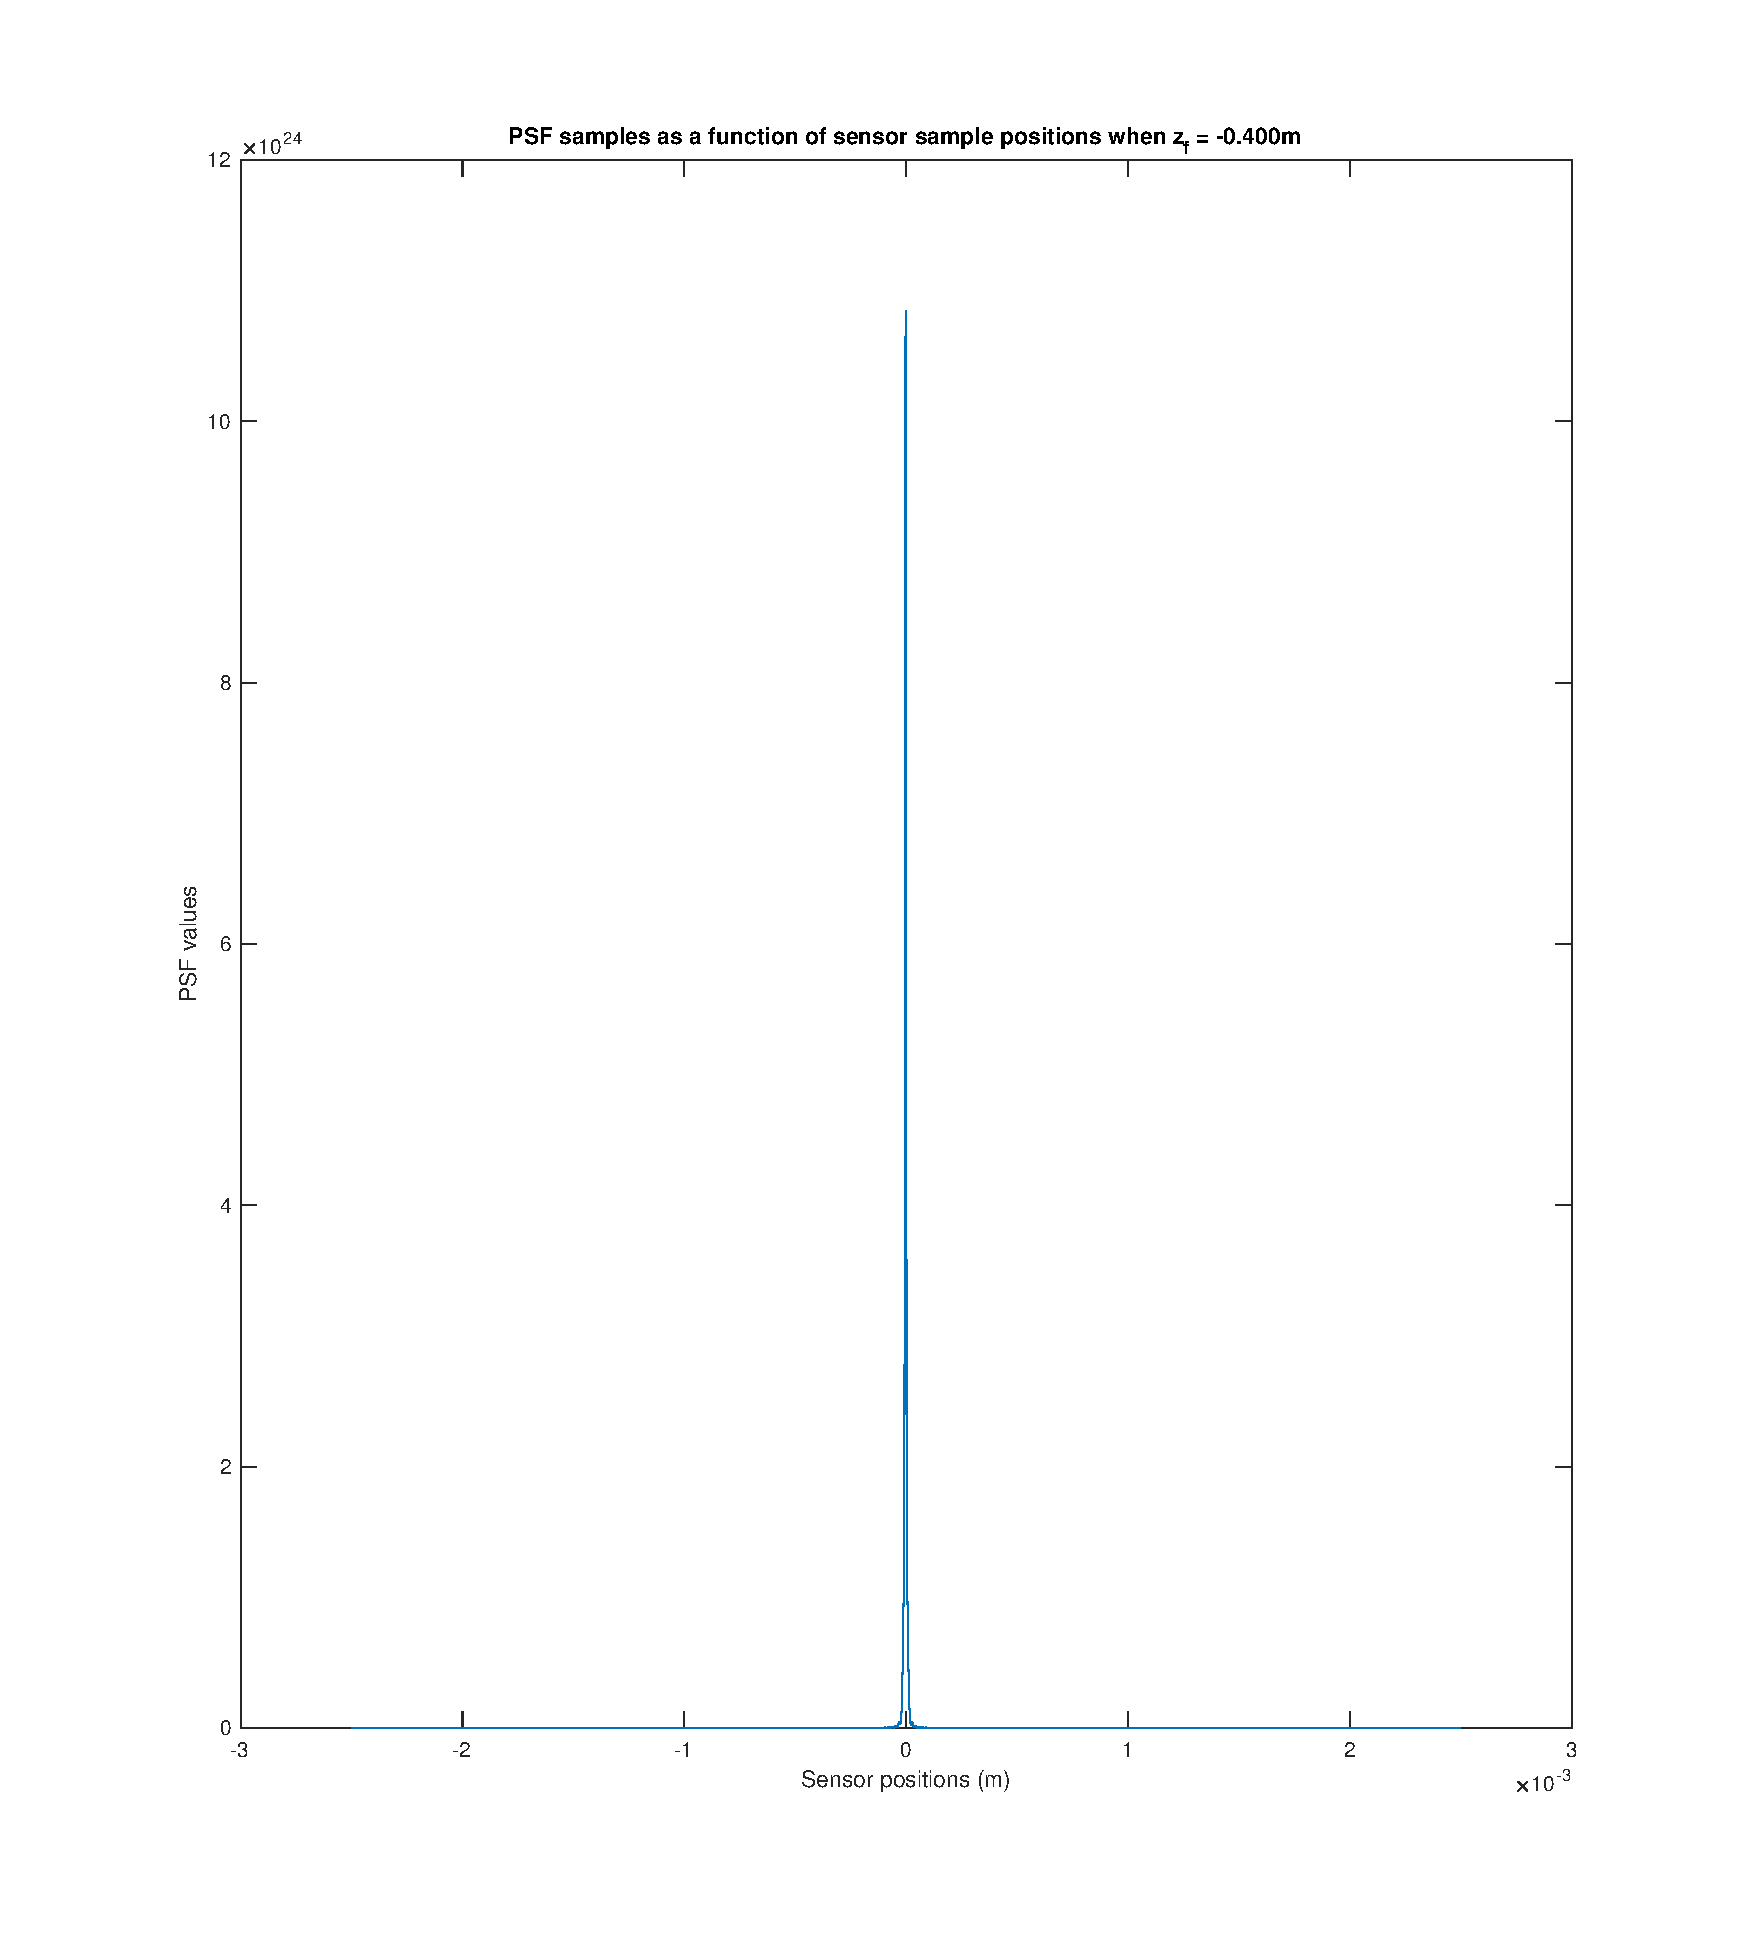
\includegraphics[width=\columnwidth]{img/psf_single_fresnel.eps}
  \caption{PSF results of the simulation with Fresnel synthesis}
  \label{fig:psf_single_fresnel}
\end{figure}

\begin{figure}
  \centering
  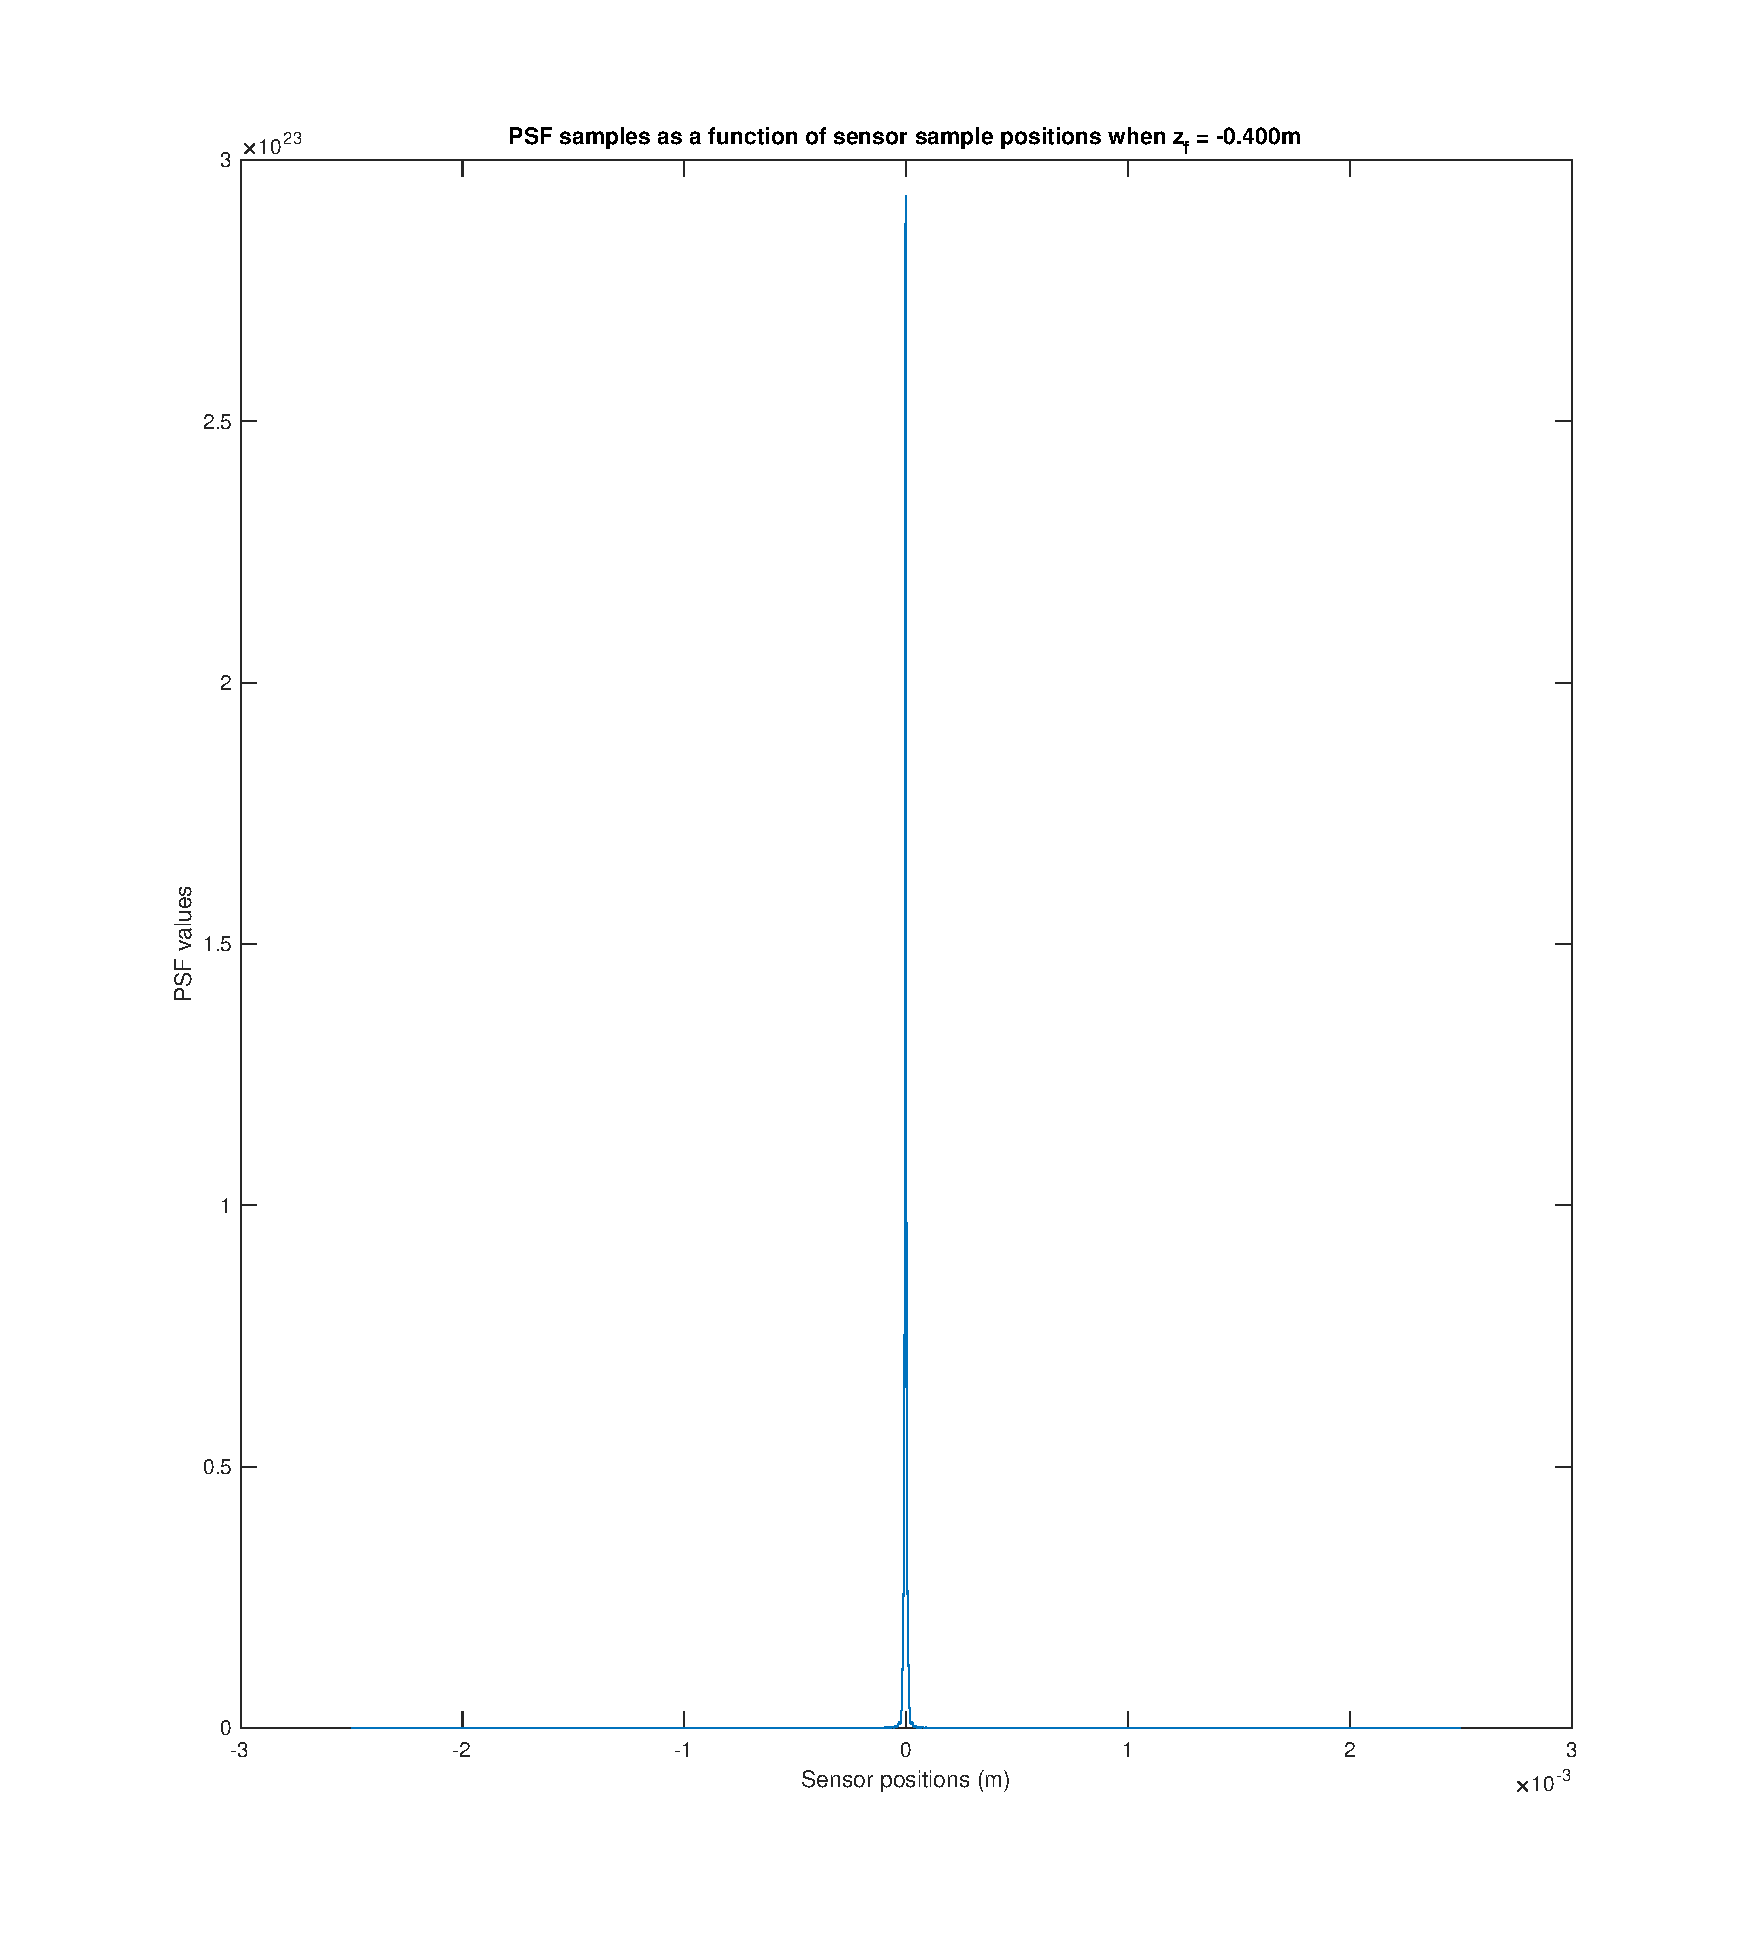
\includegraphics[width=\columnwidth]{img/psf_single_rs.eps}
  \caption{PSF results of the simulation with Rayleigh-Sommerfield synthesis}
  \label{fig:psf_single_rs}
\end{figure}

\begin{figure}
  \centering
  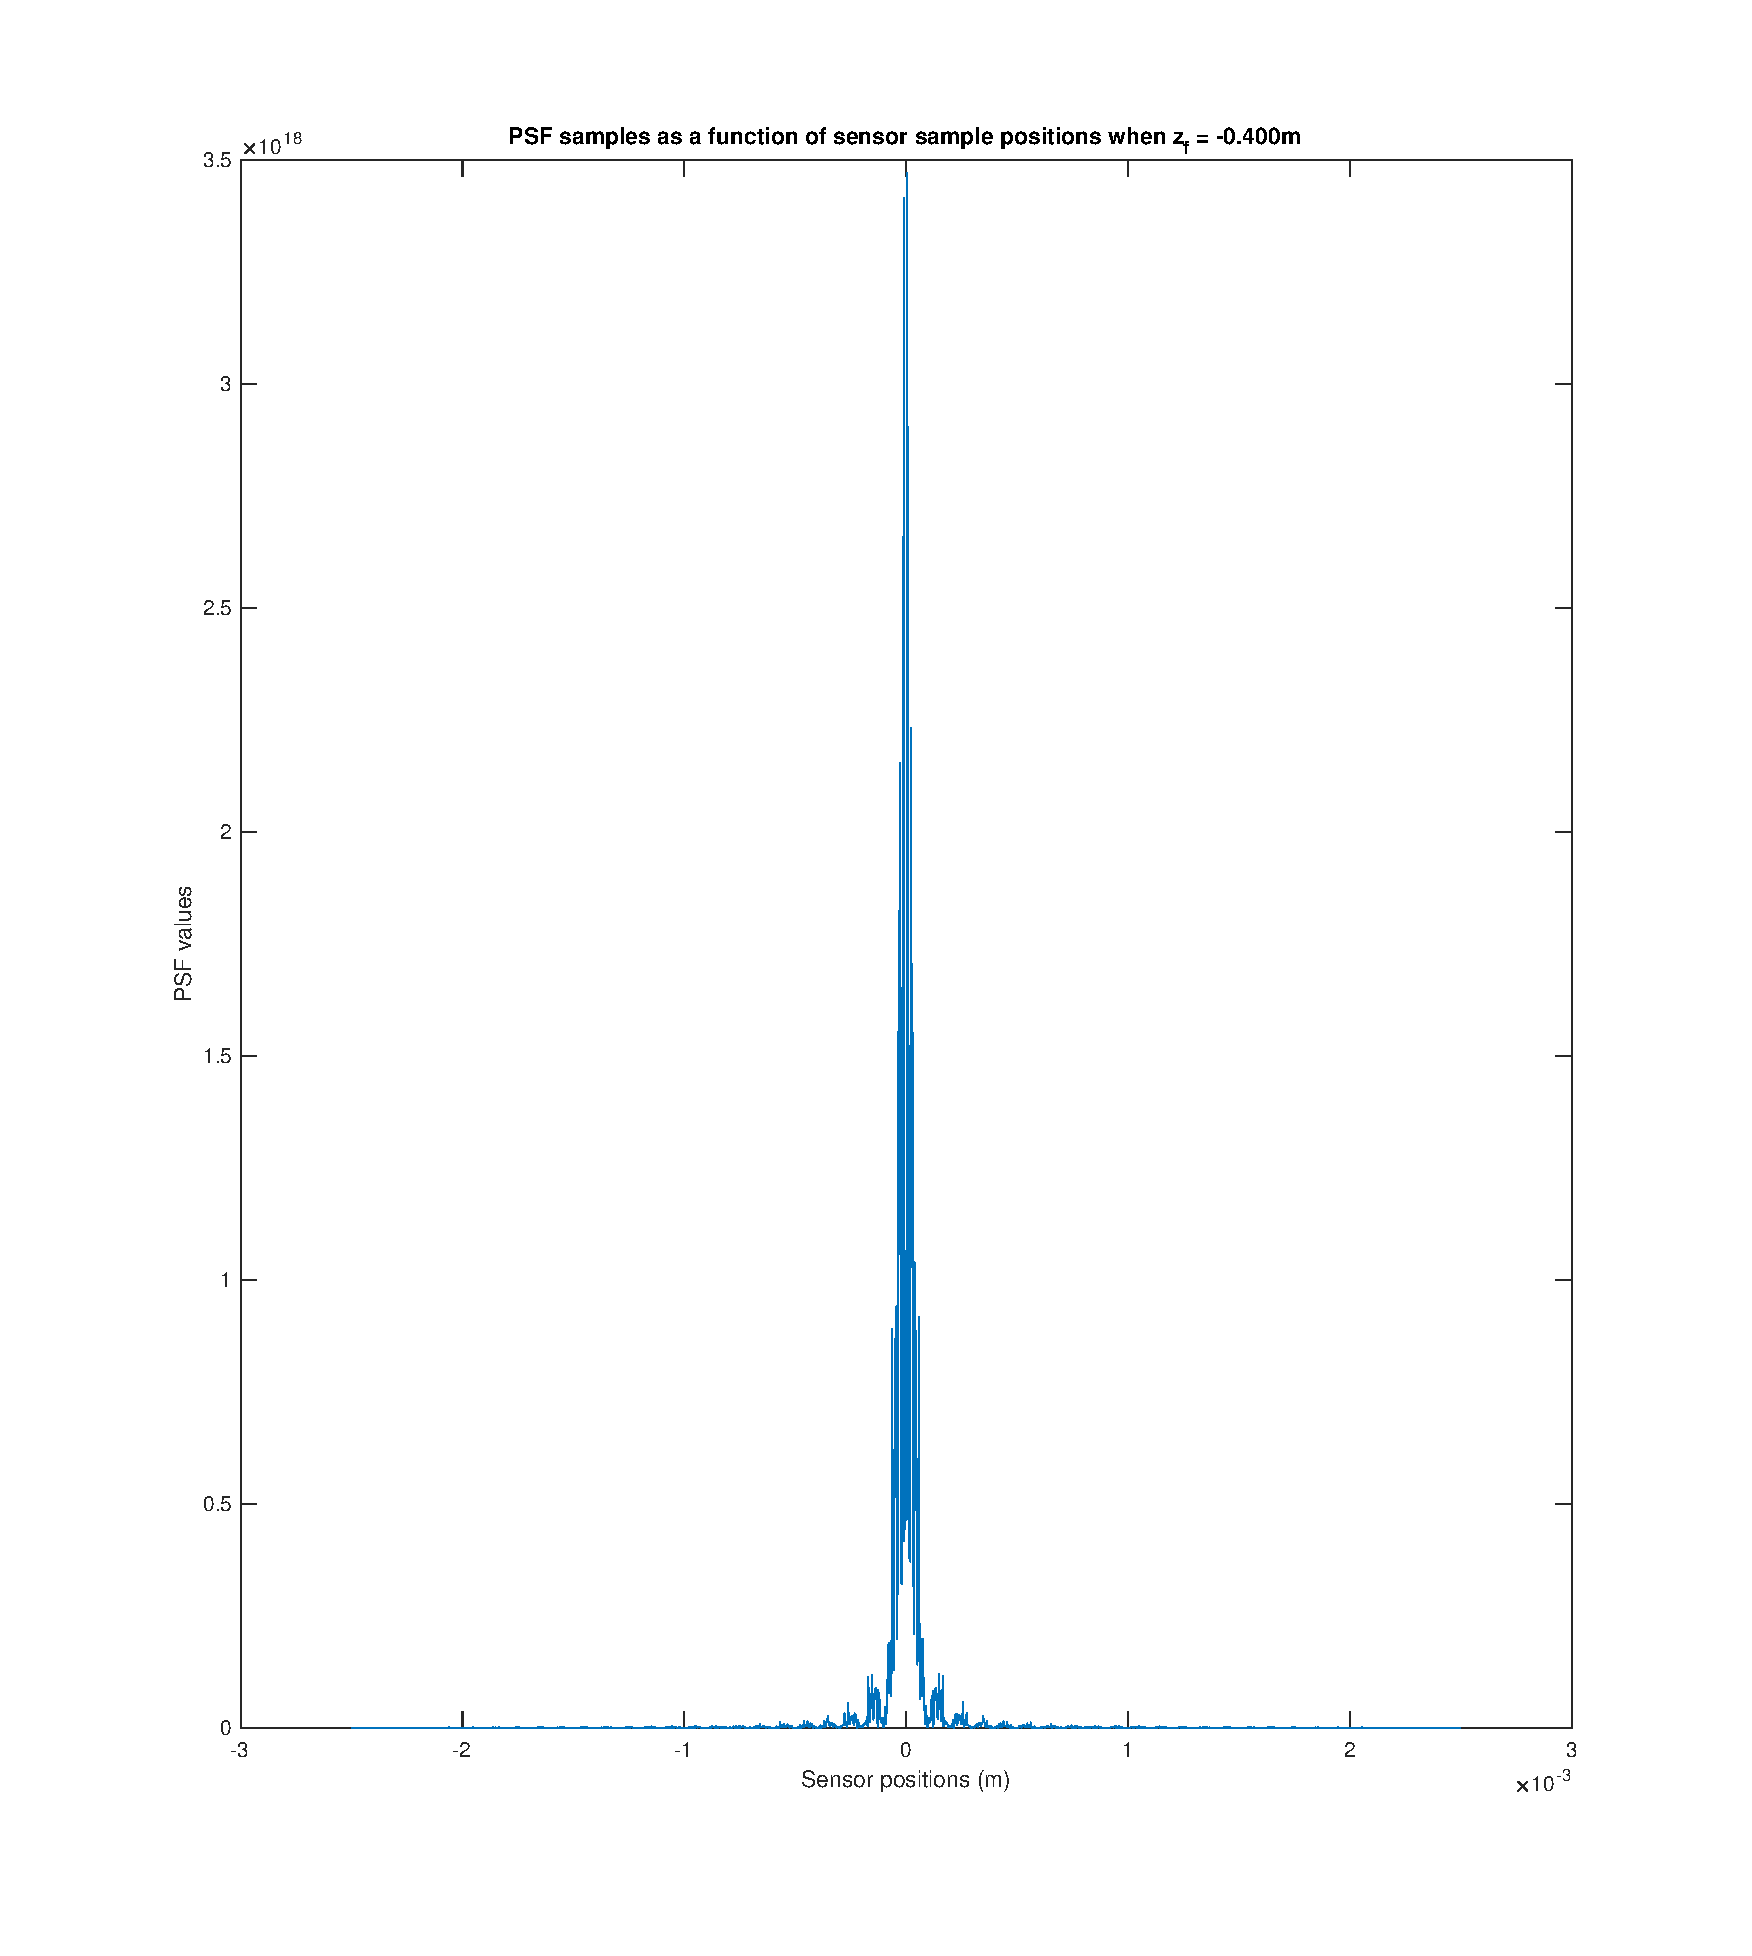
\includegraphics[width=\columnwidth]{img/psf_single_hs.eps}
  \caption{PSF results of the simulation with Holgraphic Stereopgram synthesis}
  \label{fig:psf_single_hs}
\end{figure}



\section{PSF analysis}
From the simulation we attained an image consisting of multiple overlayed PSF images depicting the hologram formed on the simulated sensor. From the image~\ref{fig:psf_multiple_fresnel} we can see that from the samples the $z_f$ value of $-0.42$ produces the sharpest image, since most of the points fall in the origin. This is different from what would be expected, since in ideal situation the sharpest images should form with the same values as the distance to point source, which in our simulation is $-0.4$. When the value of $z_f$ moves away from $-0.42$ we expected the graph to widen, since image formed won't be as sharp and this is reflected in the figure, as the values closer to $-0.42$ produce higher graphs.

We also repeated this for Rayleigh-Sommerfield synthesis and Holographic stereogram synthesis, as shown in figures~\ref{fig:psf_multiple_rs} and~\ref{fig:psf_multiple_hs}. The result for the Rayleigh-Sommerfield synthesis we basically identical, as the sharpest image, was obtained with the value of $-0.42$ and further away values produced wider graphs.

As for the holographic stereogram, the results different, in the sense that the sharpest image was produced with a $z_f$ value of $-0.44$. Also all the $z_f$ values produced blurrier images as the graphs were wider. This would indicate that the holographic stereogram produces overall blurrier holograms.

\begin{figure}
  \centering
  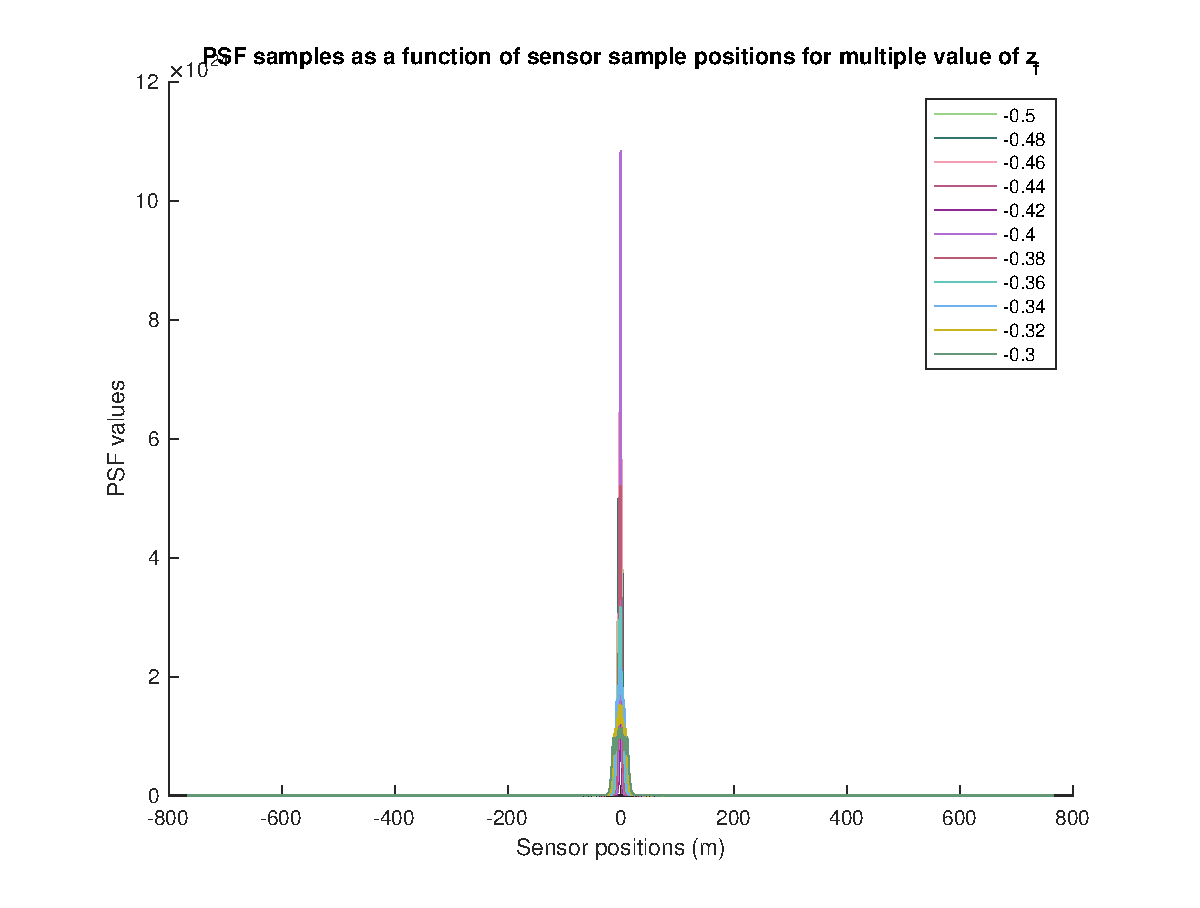
\includegraphics[width=\columnwidth]{img/psf_multiple_fresnel.eps}
  \caption{PSF results of the simulation with Fresnel synthesis, with multiple $z_f$ values between $-0.5$ and $-0.3$}
  \label{fig:psf_multiple_fresnel}
\end{figure}

\begin{figure}
  \centering
  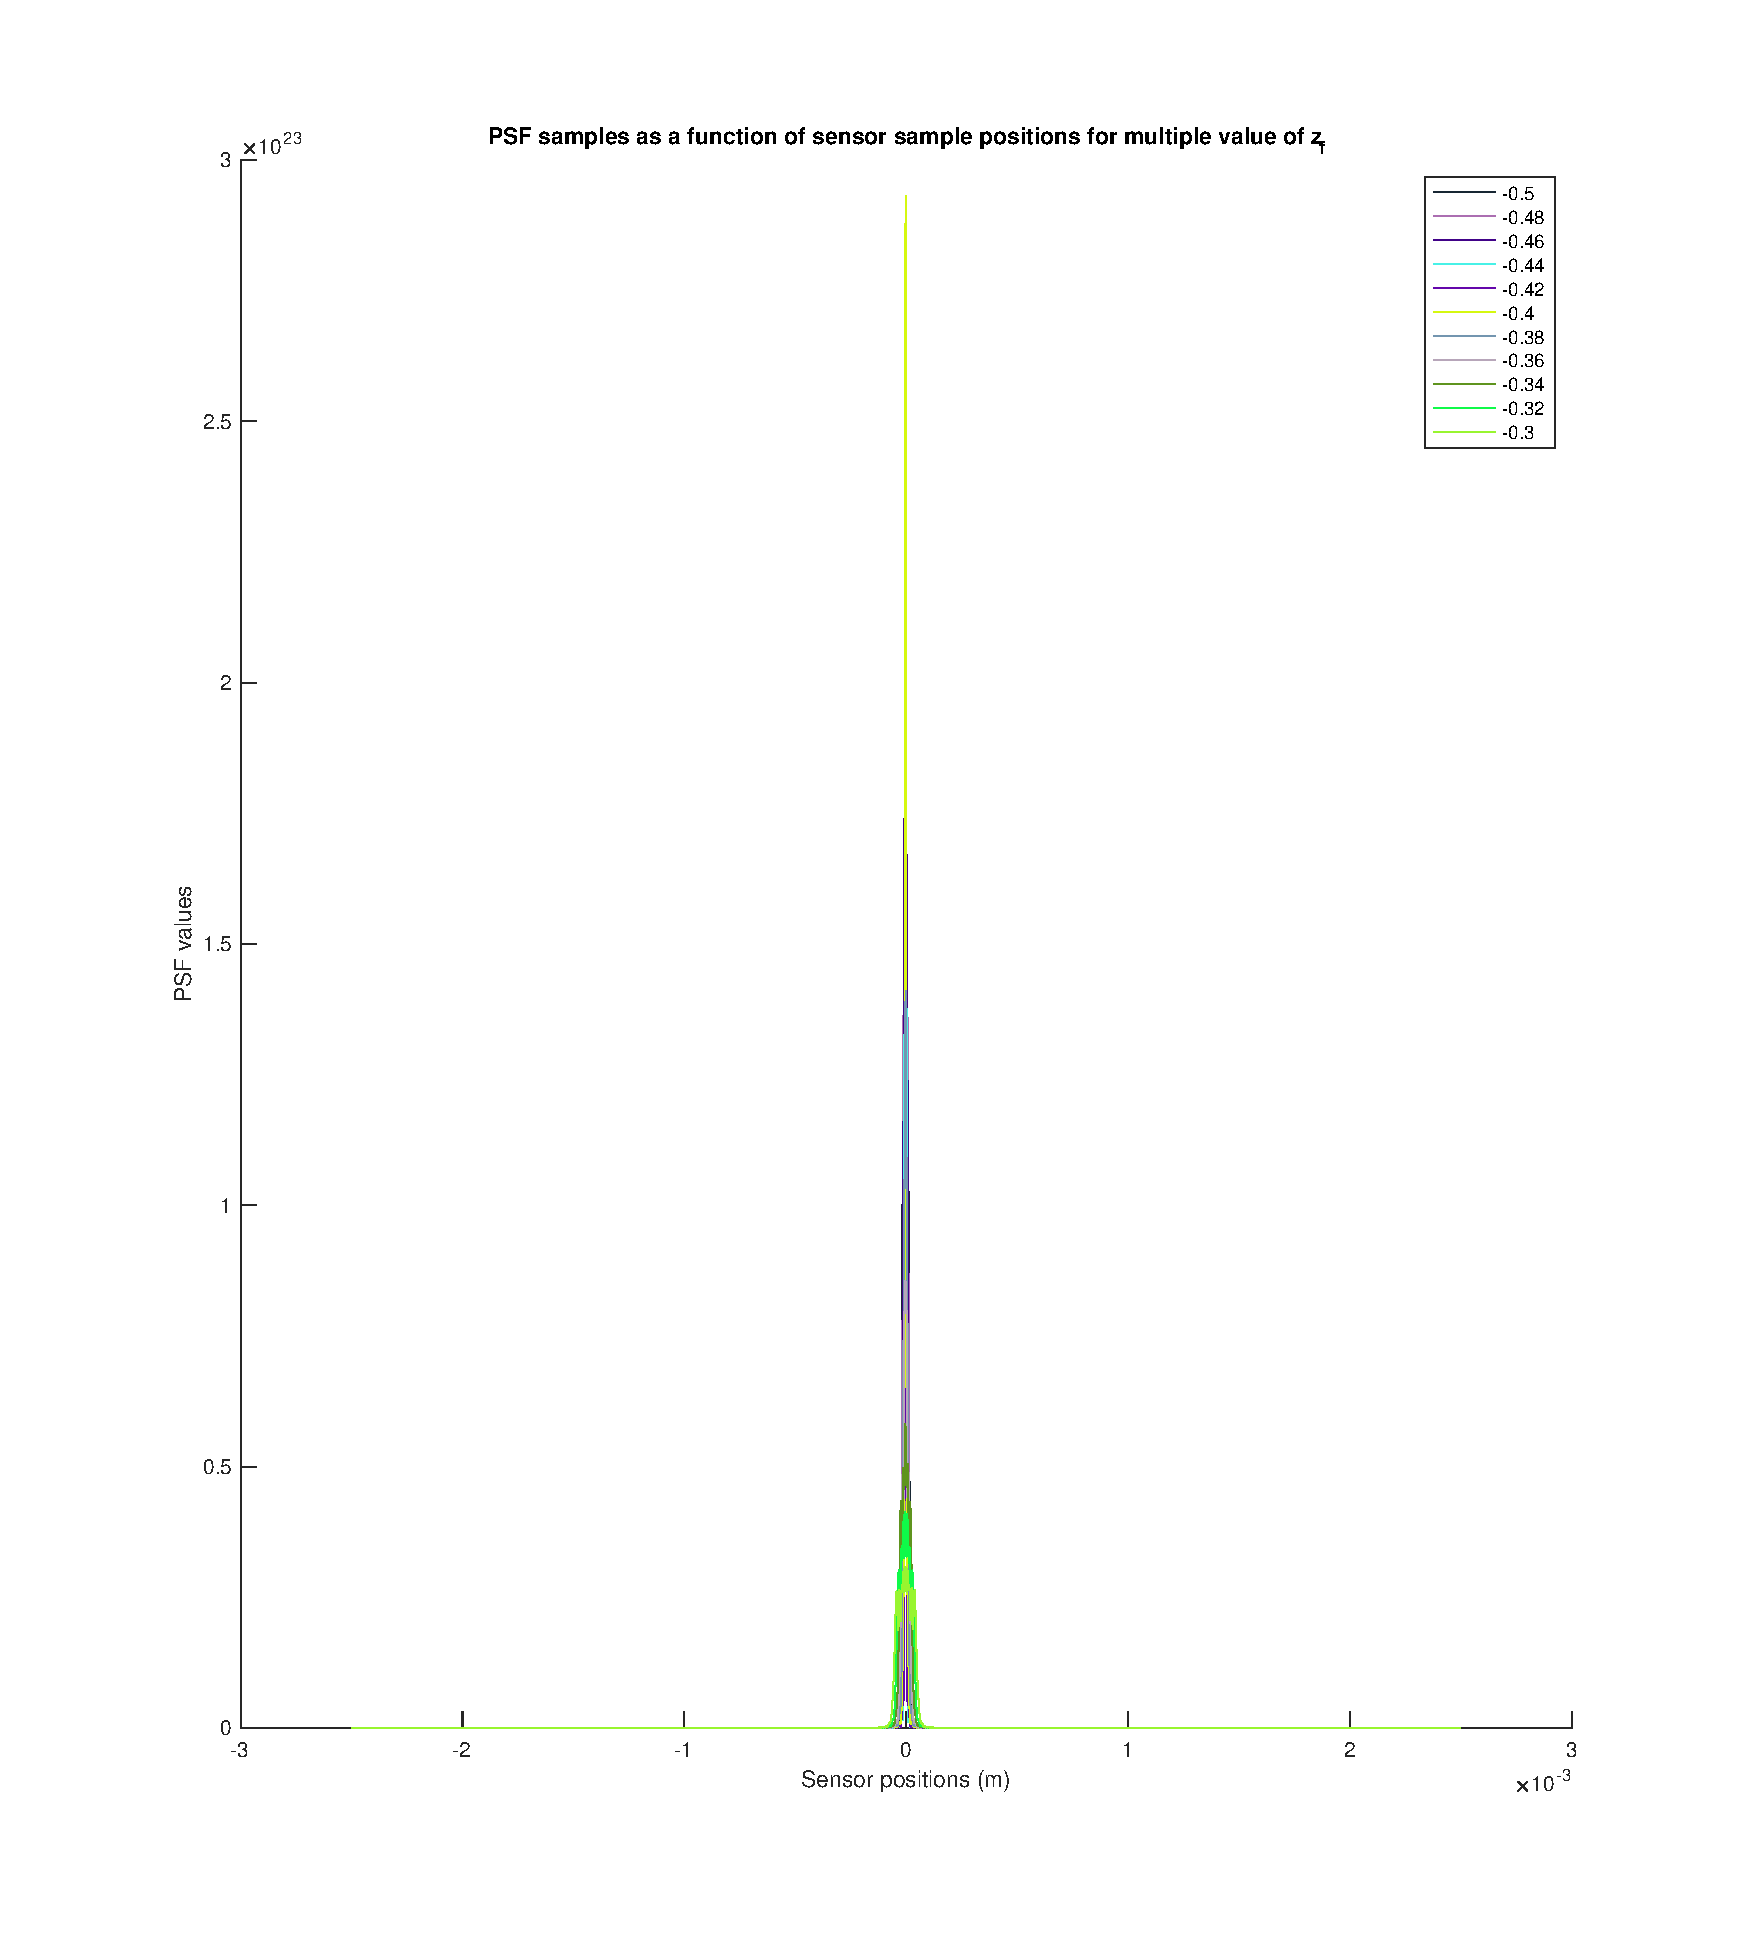
\includegraphics[width=\columnwidth]{img/psf_multiple_rs.eps}
  \caption{PSF results of the simulation with Rayleigh-Sommerfield synthesis, with multiple $z_f$ values between $-0.5$ and $-0.3$}
  \label{fig:psf_multiple_rs}
\end{figure}

\begin{figure}
  \centering
  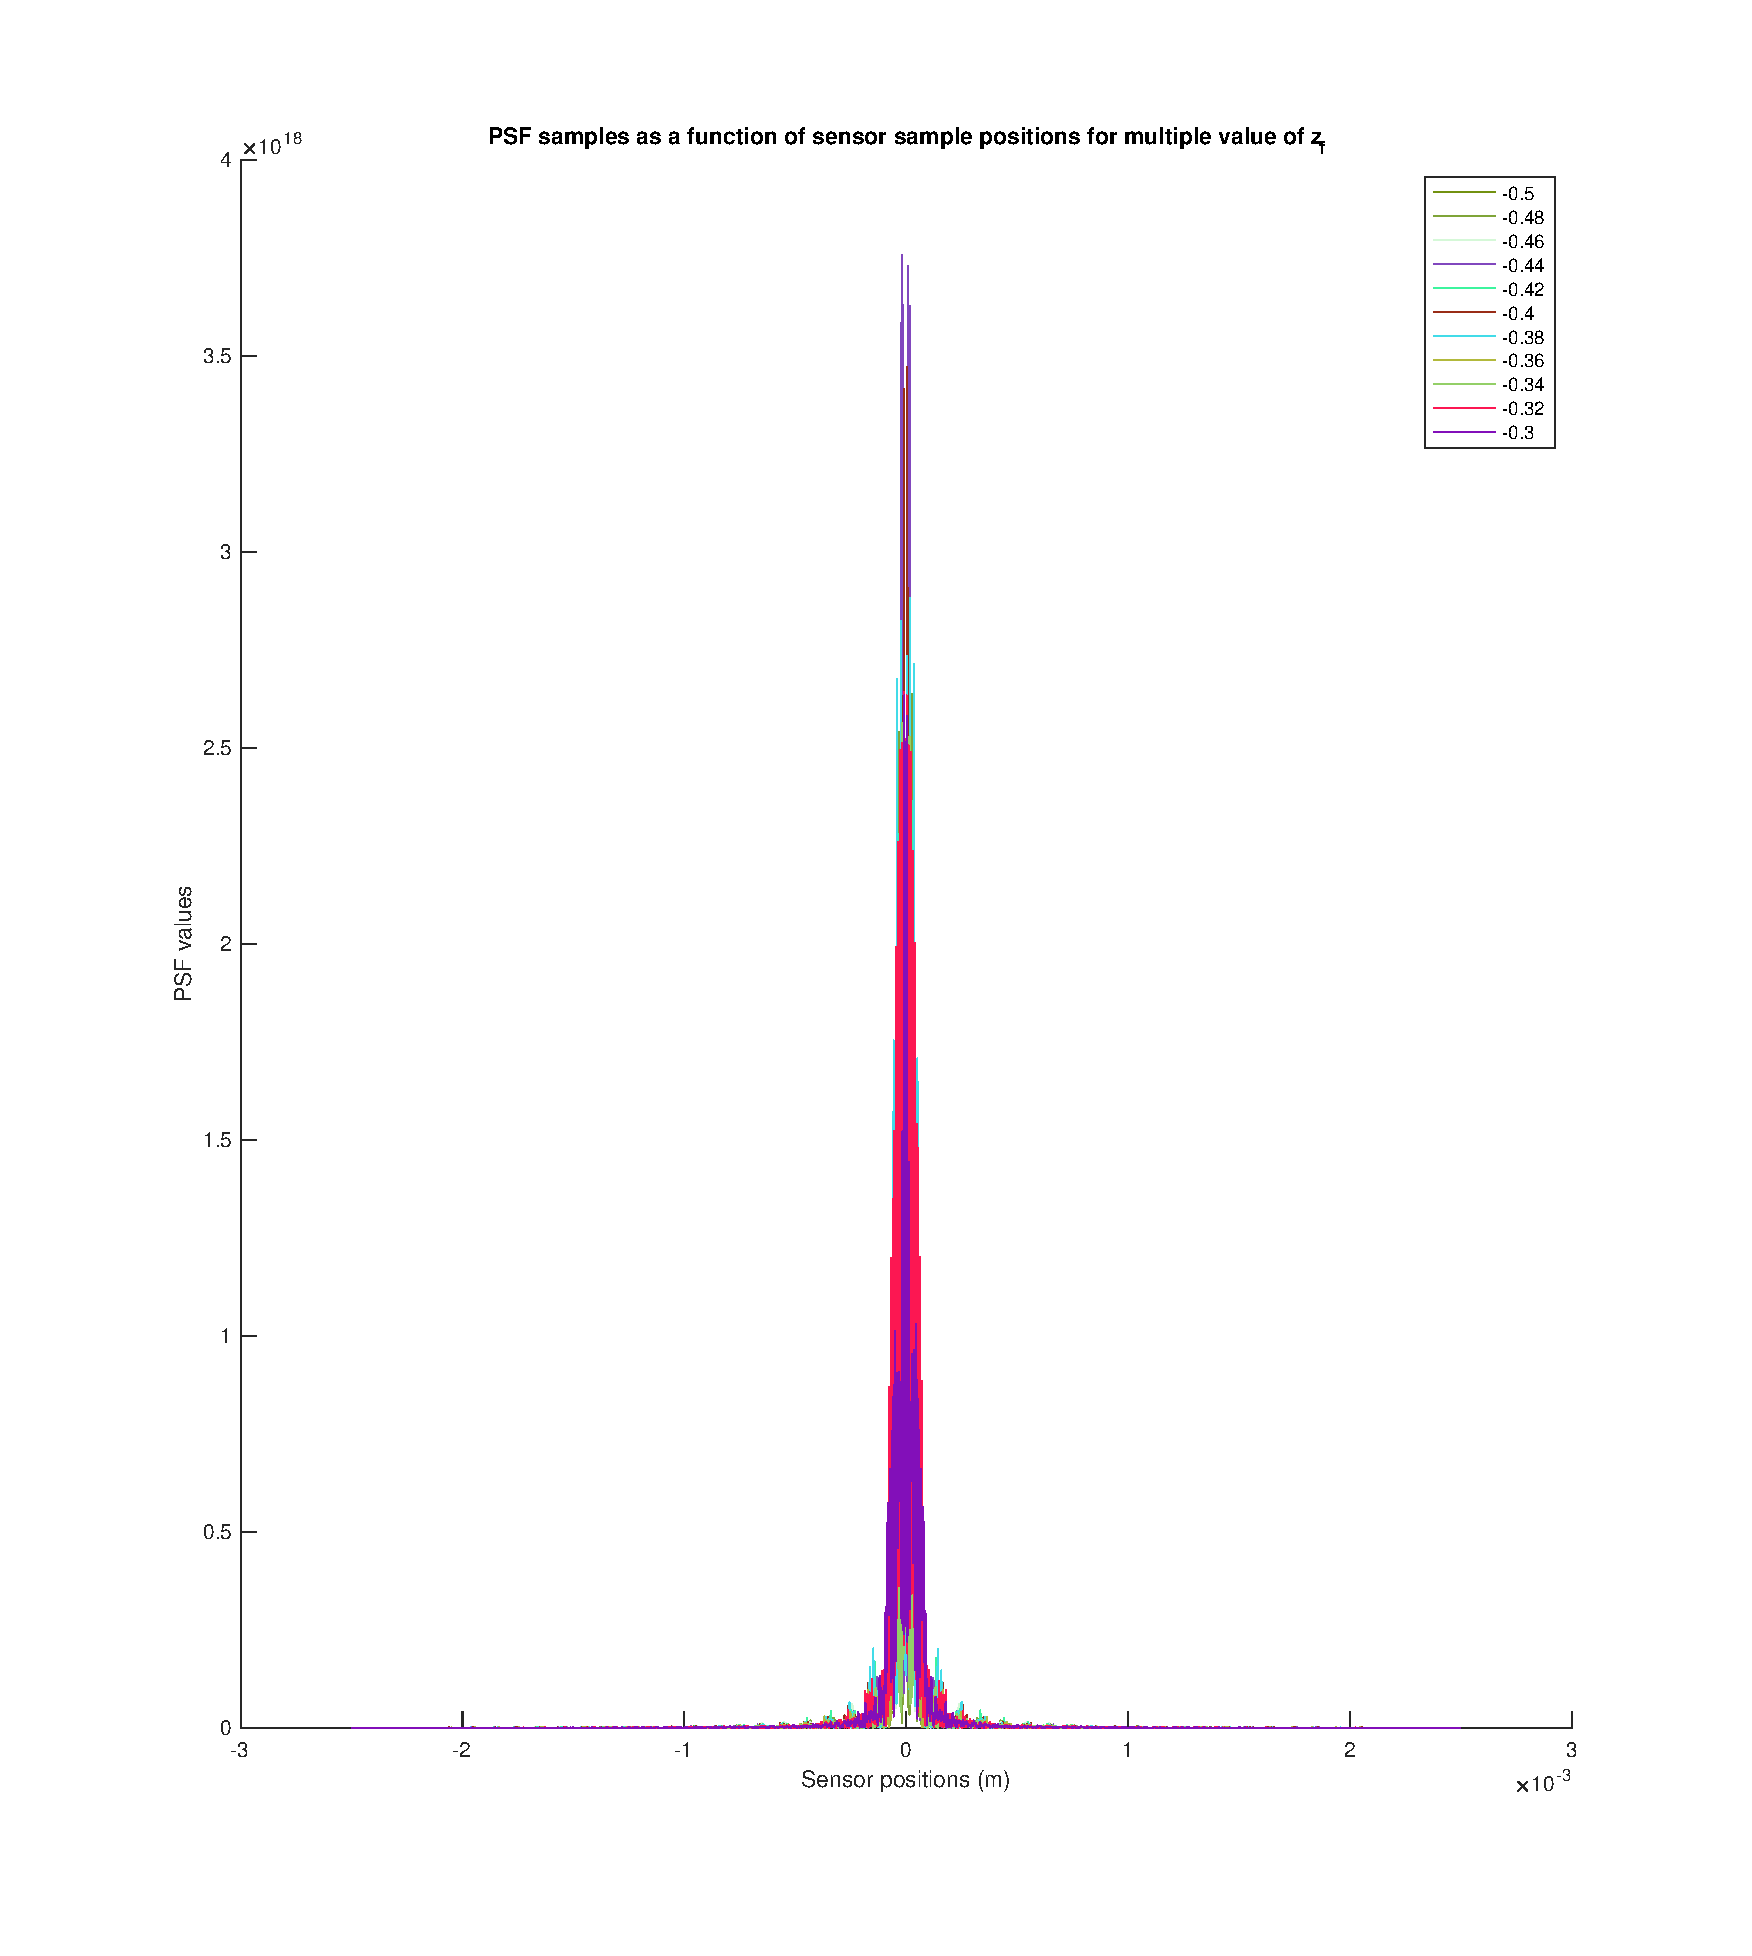
\includegraphics[width=\columnwidth]{img/psf_multiple_hs.eps}
  \caption{PSF results of the simulation with holograpic stereograph synthesis, with multiple $z_f$ values between $-0.5$ and $-0.3$}
  \label{fig:psf_multiple_hs}
\end{figure}

\section{MTF Analysis}
With the multiple PSF images we performed MTF analysis to obtain the value of $z_f$ which would provide the sharpest image. By generating multiple PSF images with different $z_f$ values we were able to obtain multiple MTF values in particular spectral frequency. We chose spectral frequency of 15 as suggested in the instructions.

We fitted a 7th degree polynomial function to datapoints of MTF values as a function of $z_f$ values. We chose to use 7th degree polynomial function, since after some experimentation, it seemed to visually be the best match for our datapoints. From the fitted function we could more confidentally determine the depth at which value of $z_f$ the image would be the sharpest. For the Fresnel and Rayleigh-Sommerield synthezied holograms the values was $-0.4190$ and for the stereogram synthesis the value was $-0.446$, as can be seen from figures~\ref{fig:mtf_fresnel}, \ref{fig:mtf_rs} and~\ref{fig:mtf_hs}.

The results where closely in line with the observations we made from the overlayed PSF images. The value optimal $z_f$ value in our system is slightly offset from the expected optimal value of $-0.4$, which corresponds to the point source of the hologarm. This offset might be caused by bad approximations in the hologram synthesis or bad assumptions during the wave field propagation. Our fitting function might not be optimal for this case. The coefficients of the fitted functions are shown in table~\ref{tab:coeffs}

\begin{table}
  \centering
  \label{tab:coeffs}
  \caption{Coefficients for 7th degree polynomial function used in MTF analysis. $a_0 + a_1*x + a_2*x^2 + a_3*x^3 ... a_7*x^7$}
\begin{tabular}{|c|c|c|c|}
  \hline
  Coefficients & Fresnel & RSS & HSS \\ \hline
  $a_0$ & $9.853*10^4$ & $9.851*10^4$ & $349.3$ \\\hline
  $a_1$ & $1.806*10^6$ & $1.805*10^4$ & $-2982$ \\\hline
  $a_2$ & $1.41*10^7$ & $1.41*10^7$ & $-9.731*10^4$ \\\hline
  $a_3$ & $6.079*10^7$ & $6.077*10^7$ & $-7.416*10^5$ \\\hline
  $a_4$ & $1.563*10^8$ & $1.562*10^8$ & $-2.741*10^6$ \\\hline
  $a_5$ & $2.395*10^8$ & $2.395*10^7$ & $-5.488*10^6$ \\\hline
  $a_6$ & $2.727*10^7$ & $2.027*10^8$ & $-5.738*10^6$ \\\hline
  $a_7$ & $7.307*10^7$ & $7.305*10^7$ & $-2.464*10^6$ \\
  \hline
\end{tabular}
\end{table}




\begin{figure}
  \centering
  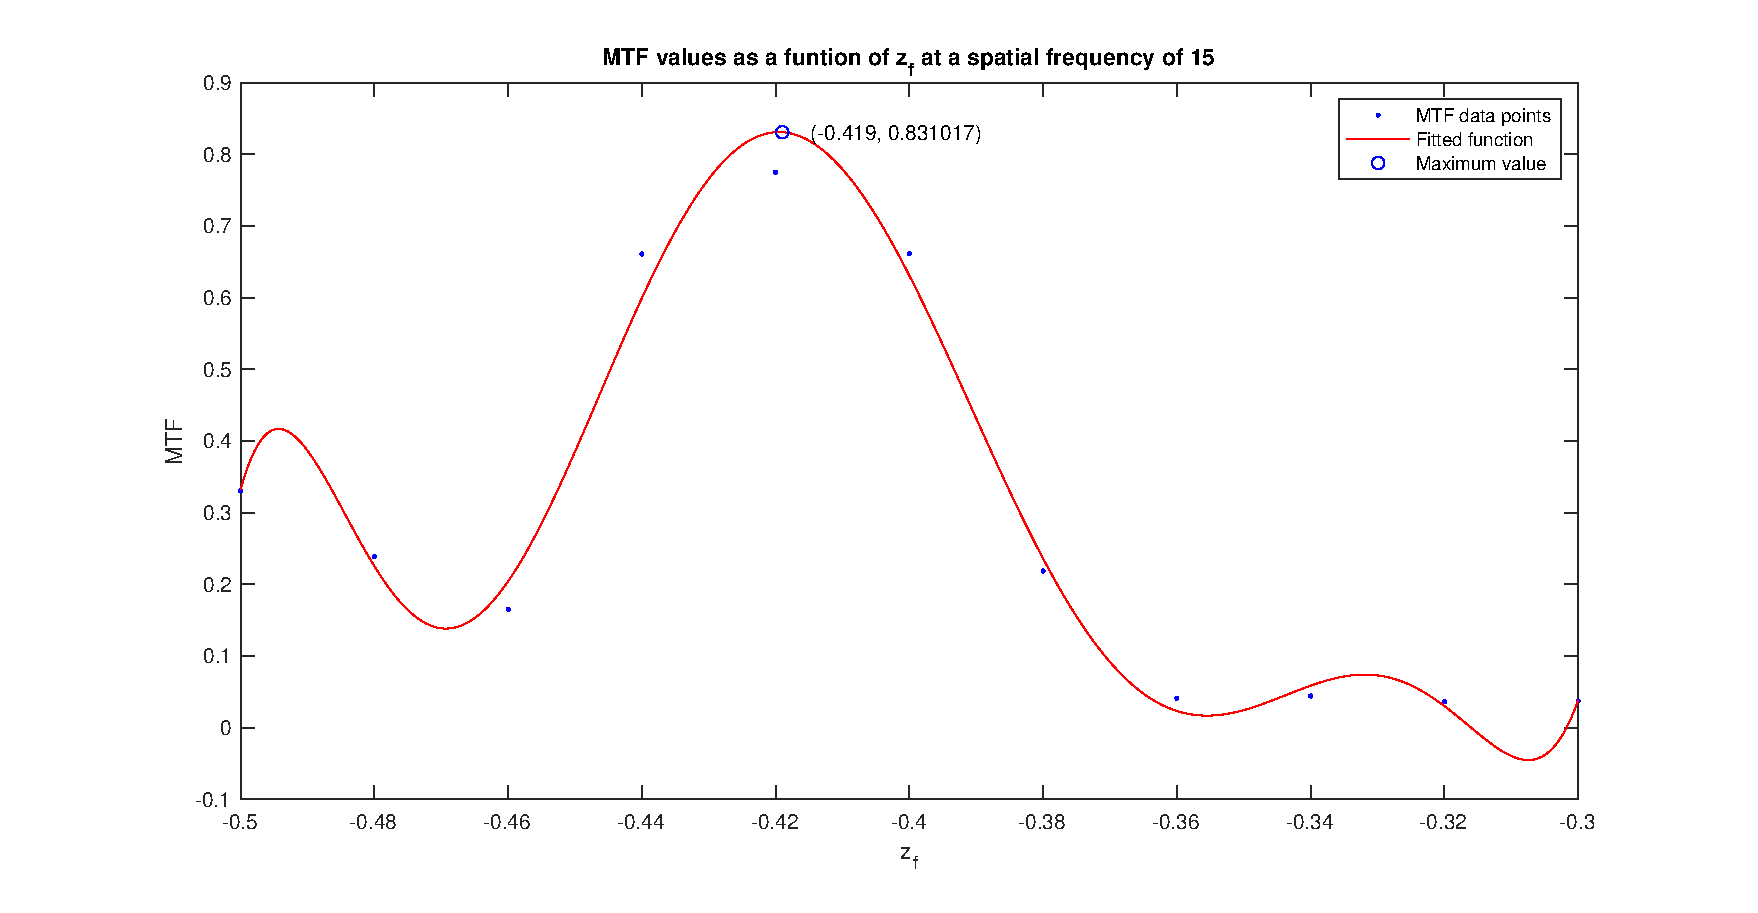
\includegraphics[width=\columnwidth]{img/mtf_fresnel.eps}
  \caption{MTF analysis results for Fresnel synthesis}
  \label{fig:mtf_fresnel}
\end{figure}

\begin{figure}
  \centering
  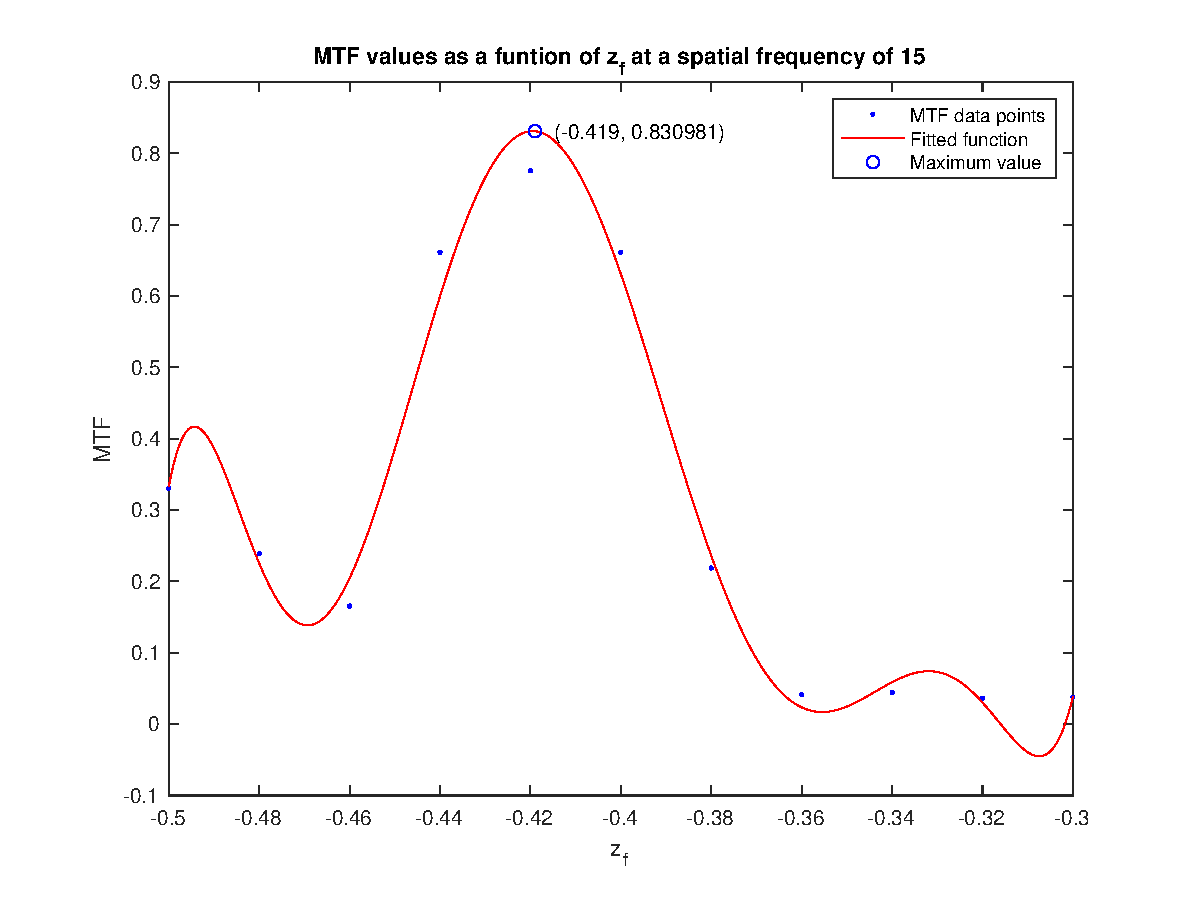
\includegraphics[width=\columnwidth]{img/mtf_rs.eps}
  \caption{MTF analysis results for Rayleigh-Sommerfield synthesis}
  \label{fig:mtf_rs}
\end{figure}

\begin{figure}
  \centering
  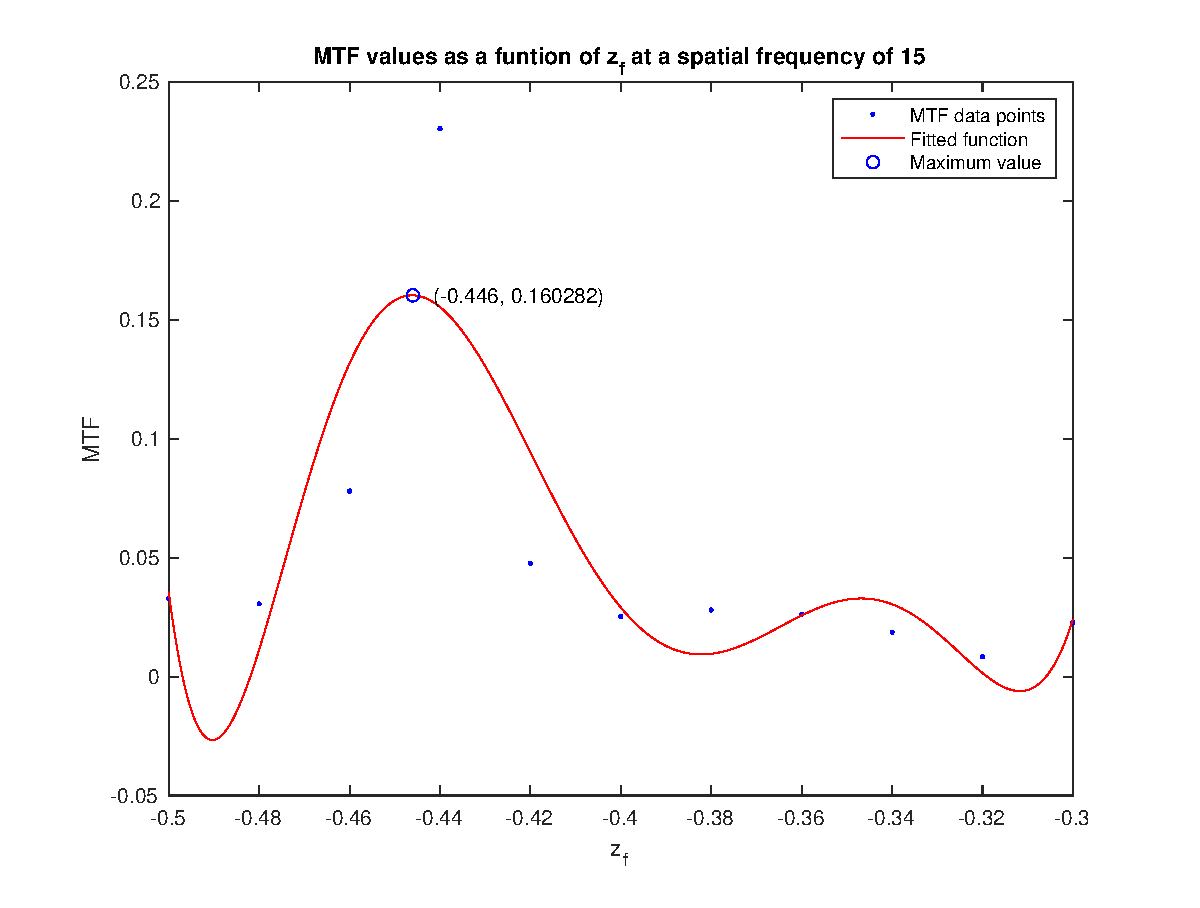
\includegraphics[width=\columnwidth]{img/mtf_hs.eps}
  \caption{MTF analysis results for Holographic stereograph synthesis}
  \label{fig:mtf_hs}
\end{figure}


\chapter{Conclusions}
This report described the work done for `Characterizing holographic displays via
numerical simulations` laboratory assignment. During which we learned about basics of holographics synthesis and wave field propagation, by implementing a Frensel synthesis and Rayleigh-Sommerfield synthesis methods in MATLAB as a part of hologram viewing simulation, as well as examining an existing implementation of holographic stereogram synthesis method. We used PSF image based analysis to demonstrate the differences in image quality between these methods.

Based on the analysis results we could conclude that for this particular simulation the Fresnel synthesis provided, the sharpest images, closely followed by the Rayleigh-Sommerfield synthesis. The holographic stereogram provided the worst results. It should be noted that these results are only applicable for this particular simulation. For example in 3D space the results might be different.

In conclusion we were able to implement the required functionality in the simulation. We succesfully used the simulation to analyze the differences between three different hologram synthesis methods, and we were able to distinguish some differences between them. Finally we used PSF images and MTF images to find the optimal focal length for each of the synthesis methods for the given scene.

\label{ch:conclusions}


%
% The bibliography, i.e the list of references
%
\newpage

\printbibliography[title=References]
\addcontentsline{toc}{chapter}{References}

\end{document}

